\newpage
\section{Pianificazione}
Per migliorare lo sviluppo del progetto, il team ha deciso di suddividere il carico di lavoro in sei periodi:
\begin{itemize}
	\item \textbf{\AdR (AR)};
	\item \textbf{Analisi dei Requisiti in dettaglio (AD)};
	\item \textbf{Progettazione architetturale (PA)};
	\item \textbf{Progettazione di dettaglio (PD)};
	\item \textbf{Codifica (CO)};
	\item \textbf{Verifica e Validazione (VV)}.
\end{itemize}

Per evidenziare le attività principali di un periodo, ad ognuno di essi viene associato un diagramma di \textit{Gantt\ped{G}}. 
Ogni attività, a propria volta, può essere suddivisa in sotto-attività e fare riferimento ad una o più risorse.
Una \textit{milestone\ped{G}} può essere esterna, coincidendo con le date di consegna dei documenti, o interna, ovvero un punto di revisione stabilito dal team e all'interno di un diagramma vengono rappresentate con dei rombi neri. Il momento in cui un periodo termina coincide con una \textit{milestone\ped{G}}.\\ 
La rappresentazione temporale delle attività nel diagramma di \textit{Gantt\ped{G}} avviene mediante linee nere le cui estremità sono frecce verso il basso. 
I diagrammi di \textit{Gantt\ped{G}} permettono, grazie all'uso di frecce, di rappresentare le dipendenze tra le attività.
La conseguenza di un ritardo su un'attività è lo slittamento temporale di tutte le attività ad essa correlate . \\

Nei diagrammi \textit{Gantt\ped{G}} le sotto-attività sono suddivise nel modo seguente:
\begin{itemize}
	\item \textbf{Sotto-attività critiche}: lo svolgimento di queste attività è necessario per la riuscita del progetto nei tempi prestabiliti. Un ritardo sarebbe di grave danno per l'efficienza del team in ottica del raggiungimento della \textit{Milestone\ped{G}}. \\ 
	Le attività di questo tipo vengono rapresentate all'interno del diagramma di \textit{Gantt\ped{G}} con il colore \textit{rosso}.
	\item \textbf{Sotto-attività non critiche}: queste attività possono essere svolte parallelamente alle sotto-attività critiche. Un ritardo in tali attività non comporta un ritardo di tutto il progetto. \\
	Le attività di questo tipo vengono rapresentate all'interno del diagramma di \textit{Gantt\ped{G}} con il colore \textit{blu}.
\end{itemize}
\\
Si è deciso di non riportare i diagrammi di \textit{PERT\ped{G}} in quanto poco leggibili data la moltitudine
di nodi presenti; quindi si è scelto di presentare i soli diagrammi di \textit{Gantt\ped{G}} riportando anche le
risorse impegnate per ciascuna attività.\\

\subsection{Suddivisione delle attività}

\subsubsection{Analisi dei Requisiti}
\textbf{Periodo:} dall'8 Dicembre 2015 al 22 Gennaio 2016.\\
Questo perdiodo inizia in concomitanza alla formazione del gruppo e termina con la consegna dei documenti per la \textbf{Revisione dei Requisiti}.\\ 
Questo periodo prevede di stilare i seguenti documenti:
\begin{itemize}
		\item \textbf{Norme di Progetto}: questo è il primo documento redatto in ordine cronologico poiché norma tutto l'operato del team rigaurdo la stesura dei documenti, delle comunicazioni, etc. ed è indipendente dal capitolato scelto. E' l’Amministratore di Progetto a redigere questo documento inserendovi le norme che il team dovrà seguire durante lo svolgimento di tutte le attività. I Verificatori certificheranno che tutte le norme siano state effettivamente osservate durante le diverse attività;
		\item \textbf{Studio di Fattibilità}: in questo documento vengono analizzati tutti i capitolati proposti. Per ognuno viene analizzato il dominio tecnologico e applicativo valutandone i fattori positivi e negativi. Risulta essere un'attività	critica perché definisce il progetto sul quale il gruppo andrà a lavorare e blocca la stesura del documento di Analisi dei Requisiti;
		\item \textbf{Analisi dei Requisiti}: redatto dagli Analisti, è l'analisi approfondita del capitolato scelto con lo Studio di Fattibilità;
		\item \textbf{Piano di Progetto}: redatto dal Responsabile di Progetto, individua tutte le attività necessarie allo svolgimento del progetto e le assegna alle risorse disponibili distribuendo il carico di lavoro in maniera uniforme.
		La priorità di questo documento è alta poiché vincola tutte attività svolte dal team;
		\item \textbf{Piano di Qualifica}: steso dal Verificatore, definisce come devono essere effettuate le verifiche al fine di consegnare un prodotto di qualità;
		\item \textbf{Glossario}: scritto in maniera incrementale dai redattori dei diversi documenti e contiene la spiegazione di alcuni termini utilizzati nei vari documenti, al fine di eliminare ogni possibile ambiguità di significato;
		\item \textbf{Lettera di presentazione}: documento che dichiara l’interesse del gruppo a partecipare alla gara d’appalto.
\end{itemize}
Ogni documento sopraccitato oltre che stilato verrà anche verificato; la verifica dei presenti documenti è considerata un'attività critica.
In questa fase i ruoli maggiormente interessati sono quelli di Amministratore, Responsabile, Analista e Verificatore. 
\begin{sidewaysfigure}
	\centering
	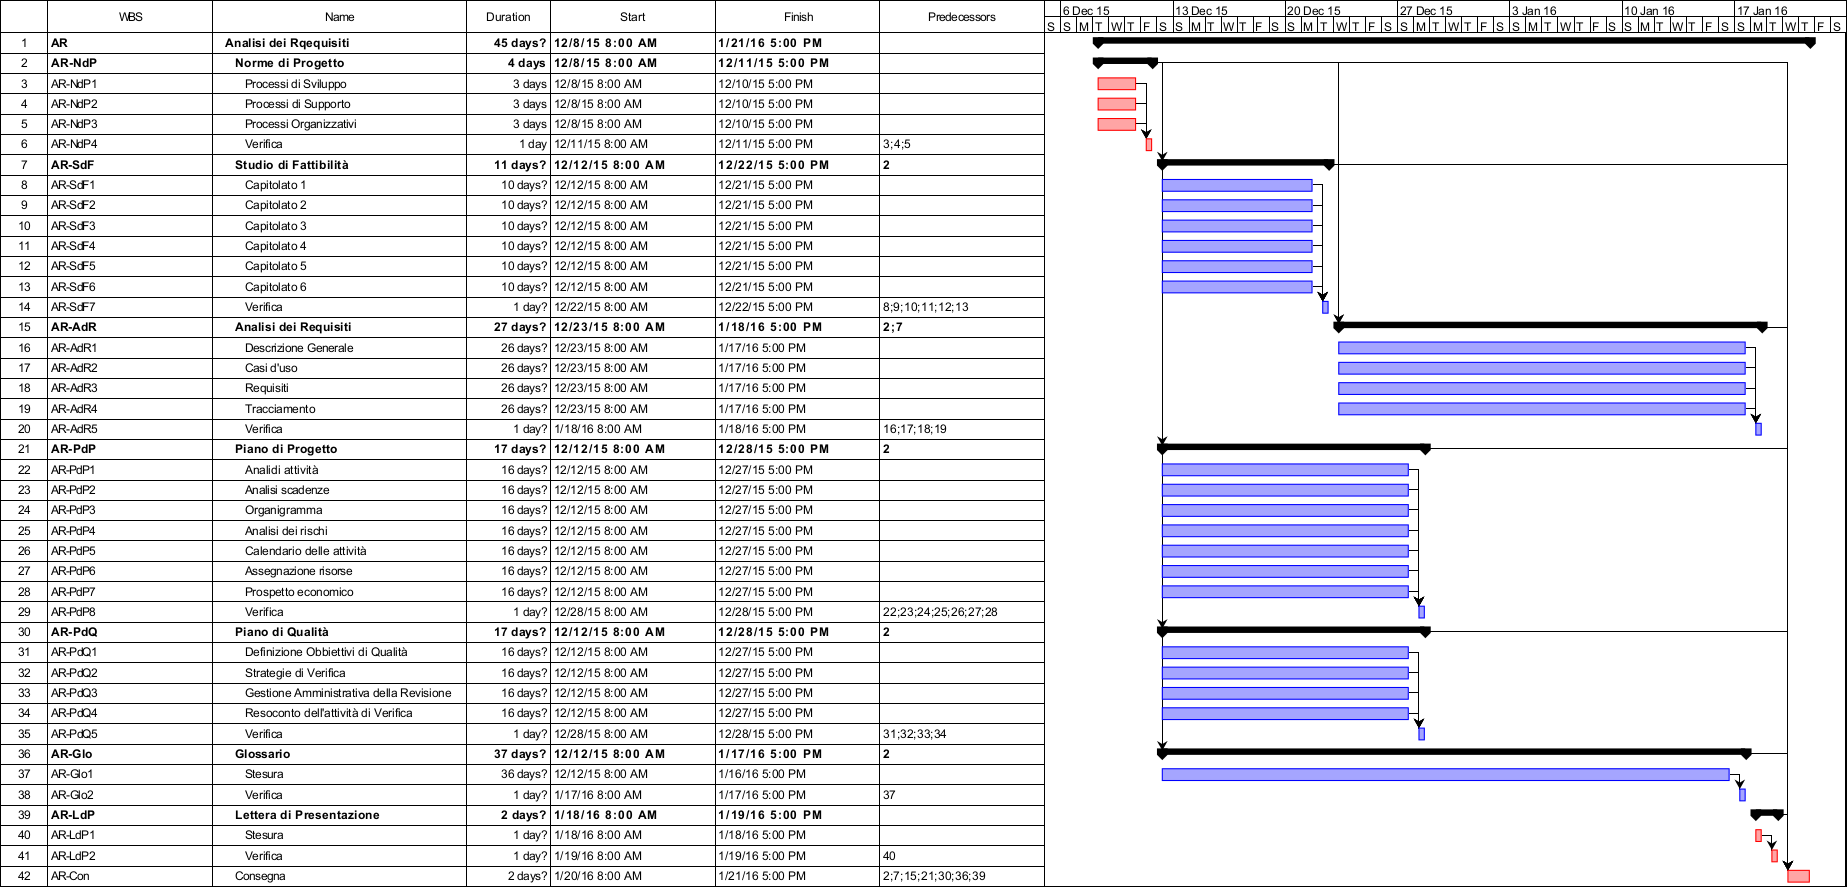
\includegraphics[keepaspectratio = true, width=23cm]{immagini/PdP_AnalisiDeiRequisitiGantt.png}
	\caption{Diagramma di Gantt relativo al periodo di Analisi dei Requisiti.}\label{etichetta}
\end{sidewaysfigure}
\newpage

\subsubsection{Analisi dei Requisiti in Dettaglio}
\textbf{Periodo:} dal 23 Gennaio 2016 al 22 Febbraio 2016. \\
Il periodo di Analisi dei Requisiti in Dettaglio inizia la consegna dei documenti per la Revisione dei Requisiti e termina con l'inizio del periodo successivo, quello della Progettazione Architturale. Il termine fissato corrisponde ad una \textit{milestone\ped{G}} interna. \\
In questo periodo il gruppo mira a consolidare ed ampliare i requisiti richiesti dal sistema e migliorare il documento di \AdR attuando le correzioni in base all'esito della Revisione dei Requisiti.
Vengono inoltre corretti e verificati anche gli altri documenti. 
 
\begin{center}
	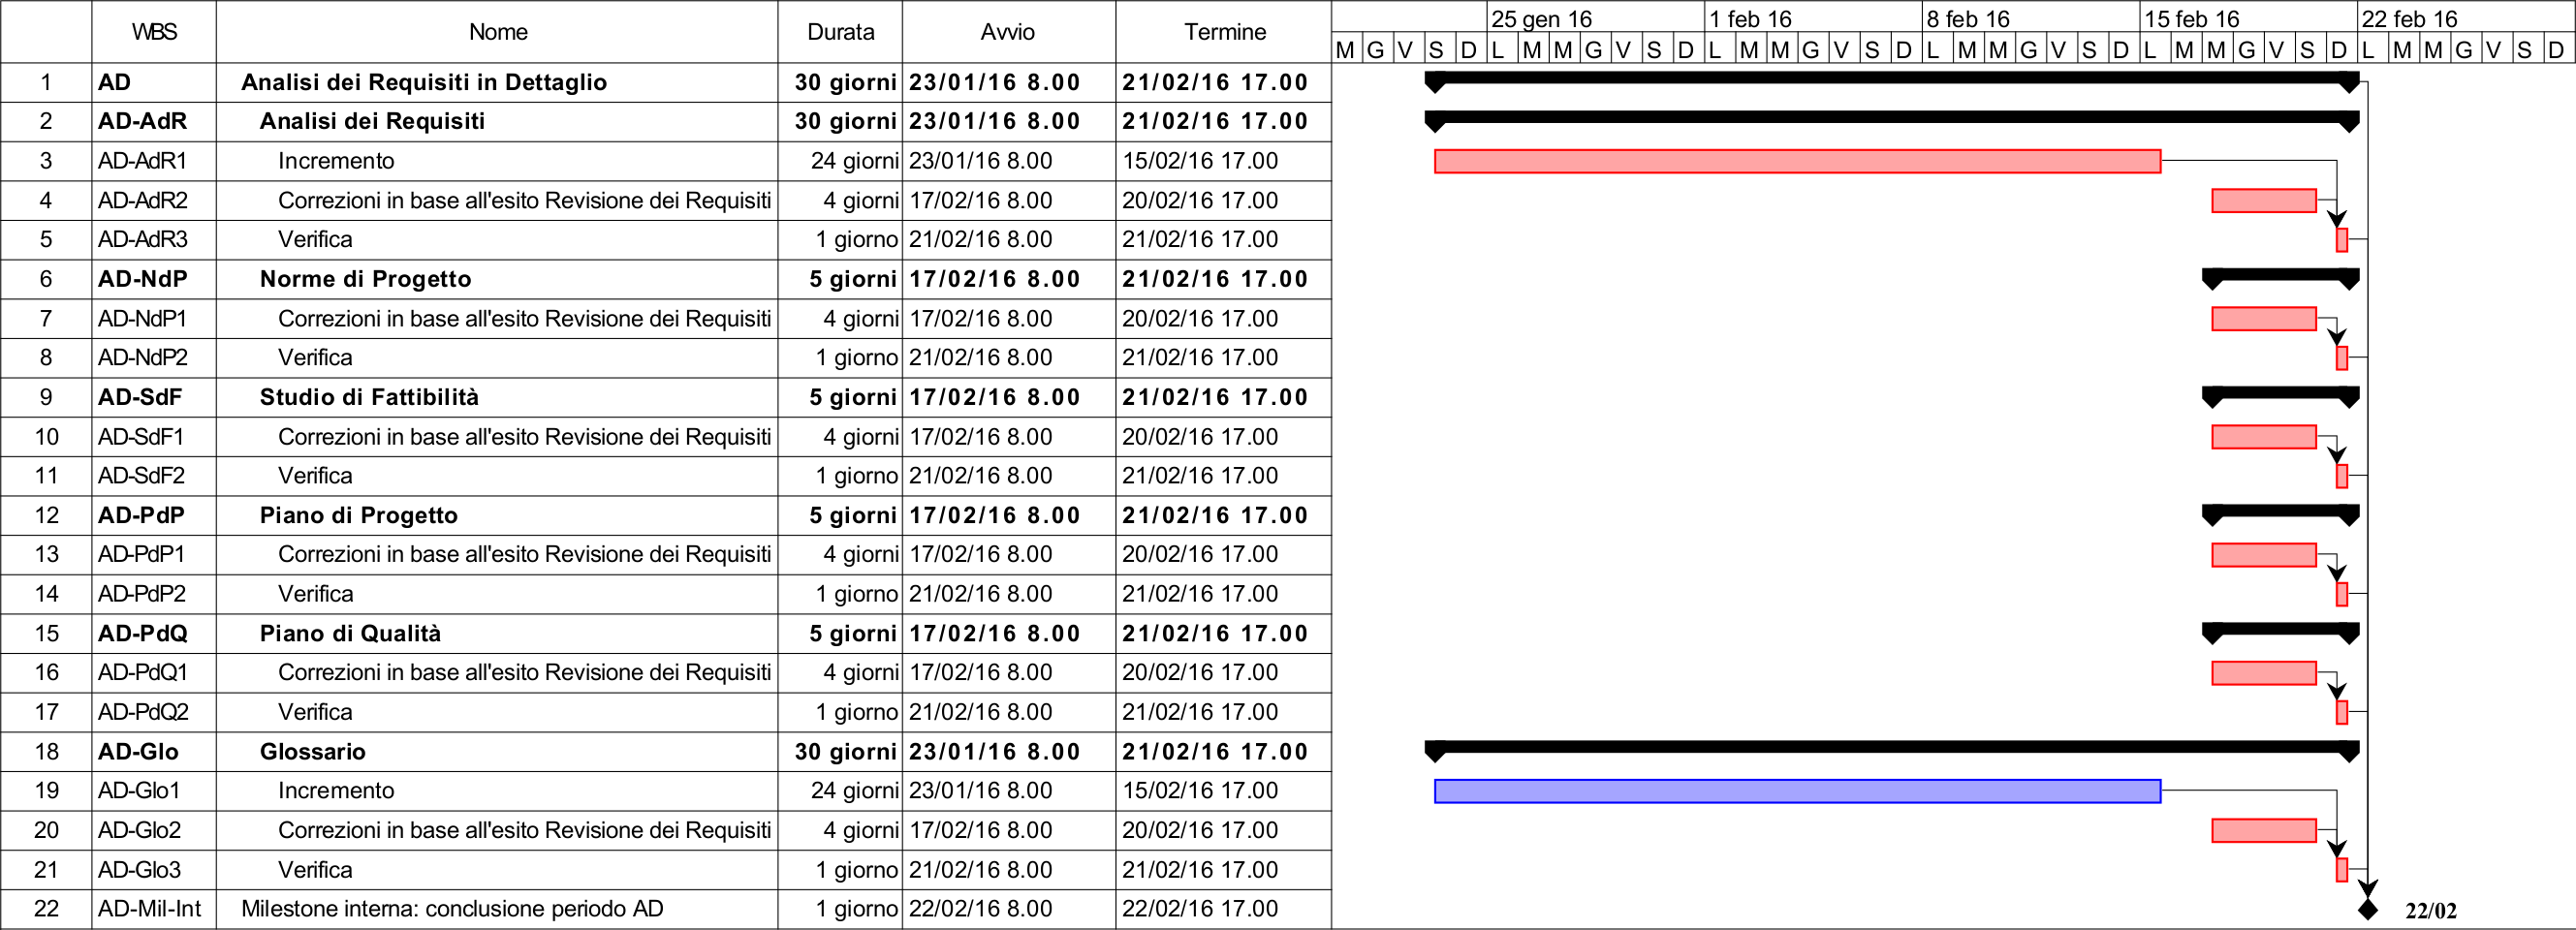
\includegraphics[keepaspectratio = true, width=16cm]{immagini/PdP_AnalisiDeiRequisitiInDettaglioGantt.png}
\end{center}
\begin{figure}[h]
	\caption{Diagramma di Gantt relativo al periodo di Analisi dei Requisiti in Dettaglio.}\label{etichetta}
\end{figure}

\subsubsection{Progettazione Architetturale}
\textbf{Periodo:} dal 23 Febbrario 2016 al 20 Marzo 2016. \\
Questo periodo, di Progettazione Architetturale, inizia dopo il periodo di Analisi dei Requisiti in Dettaglio e si conclude con una \textit{milestone\ped{G}} interna di Revisione di Progettazione minima. L'obbiettivo di questo periodo è la stesura della progettazione ad alto livello del sistema. \\
Questo periodo prevede di svolgere le seguenti attività:
\begin{itemize}
	\item Redigire il documento di \textbf{Specifica Tecnica}: il \Prog deve descrivere le scelte progettuali di alto livello effettuale, i design patter scelti per la realizzazione del prodotto e l'archittura generale del software. Inoltre deve viene effettuato il tracciamento dei requisiti.  
	\item Incrementare i documenti di \textbf{\NdP},\textbf{\PdP} e \textbf{\PdQ}.
	\item Verifica di tutti i documenti sopraccitati.
\end{itemize}
\begin{center}
	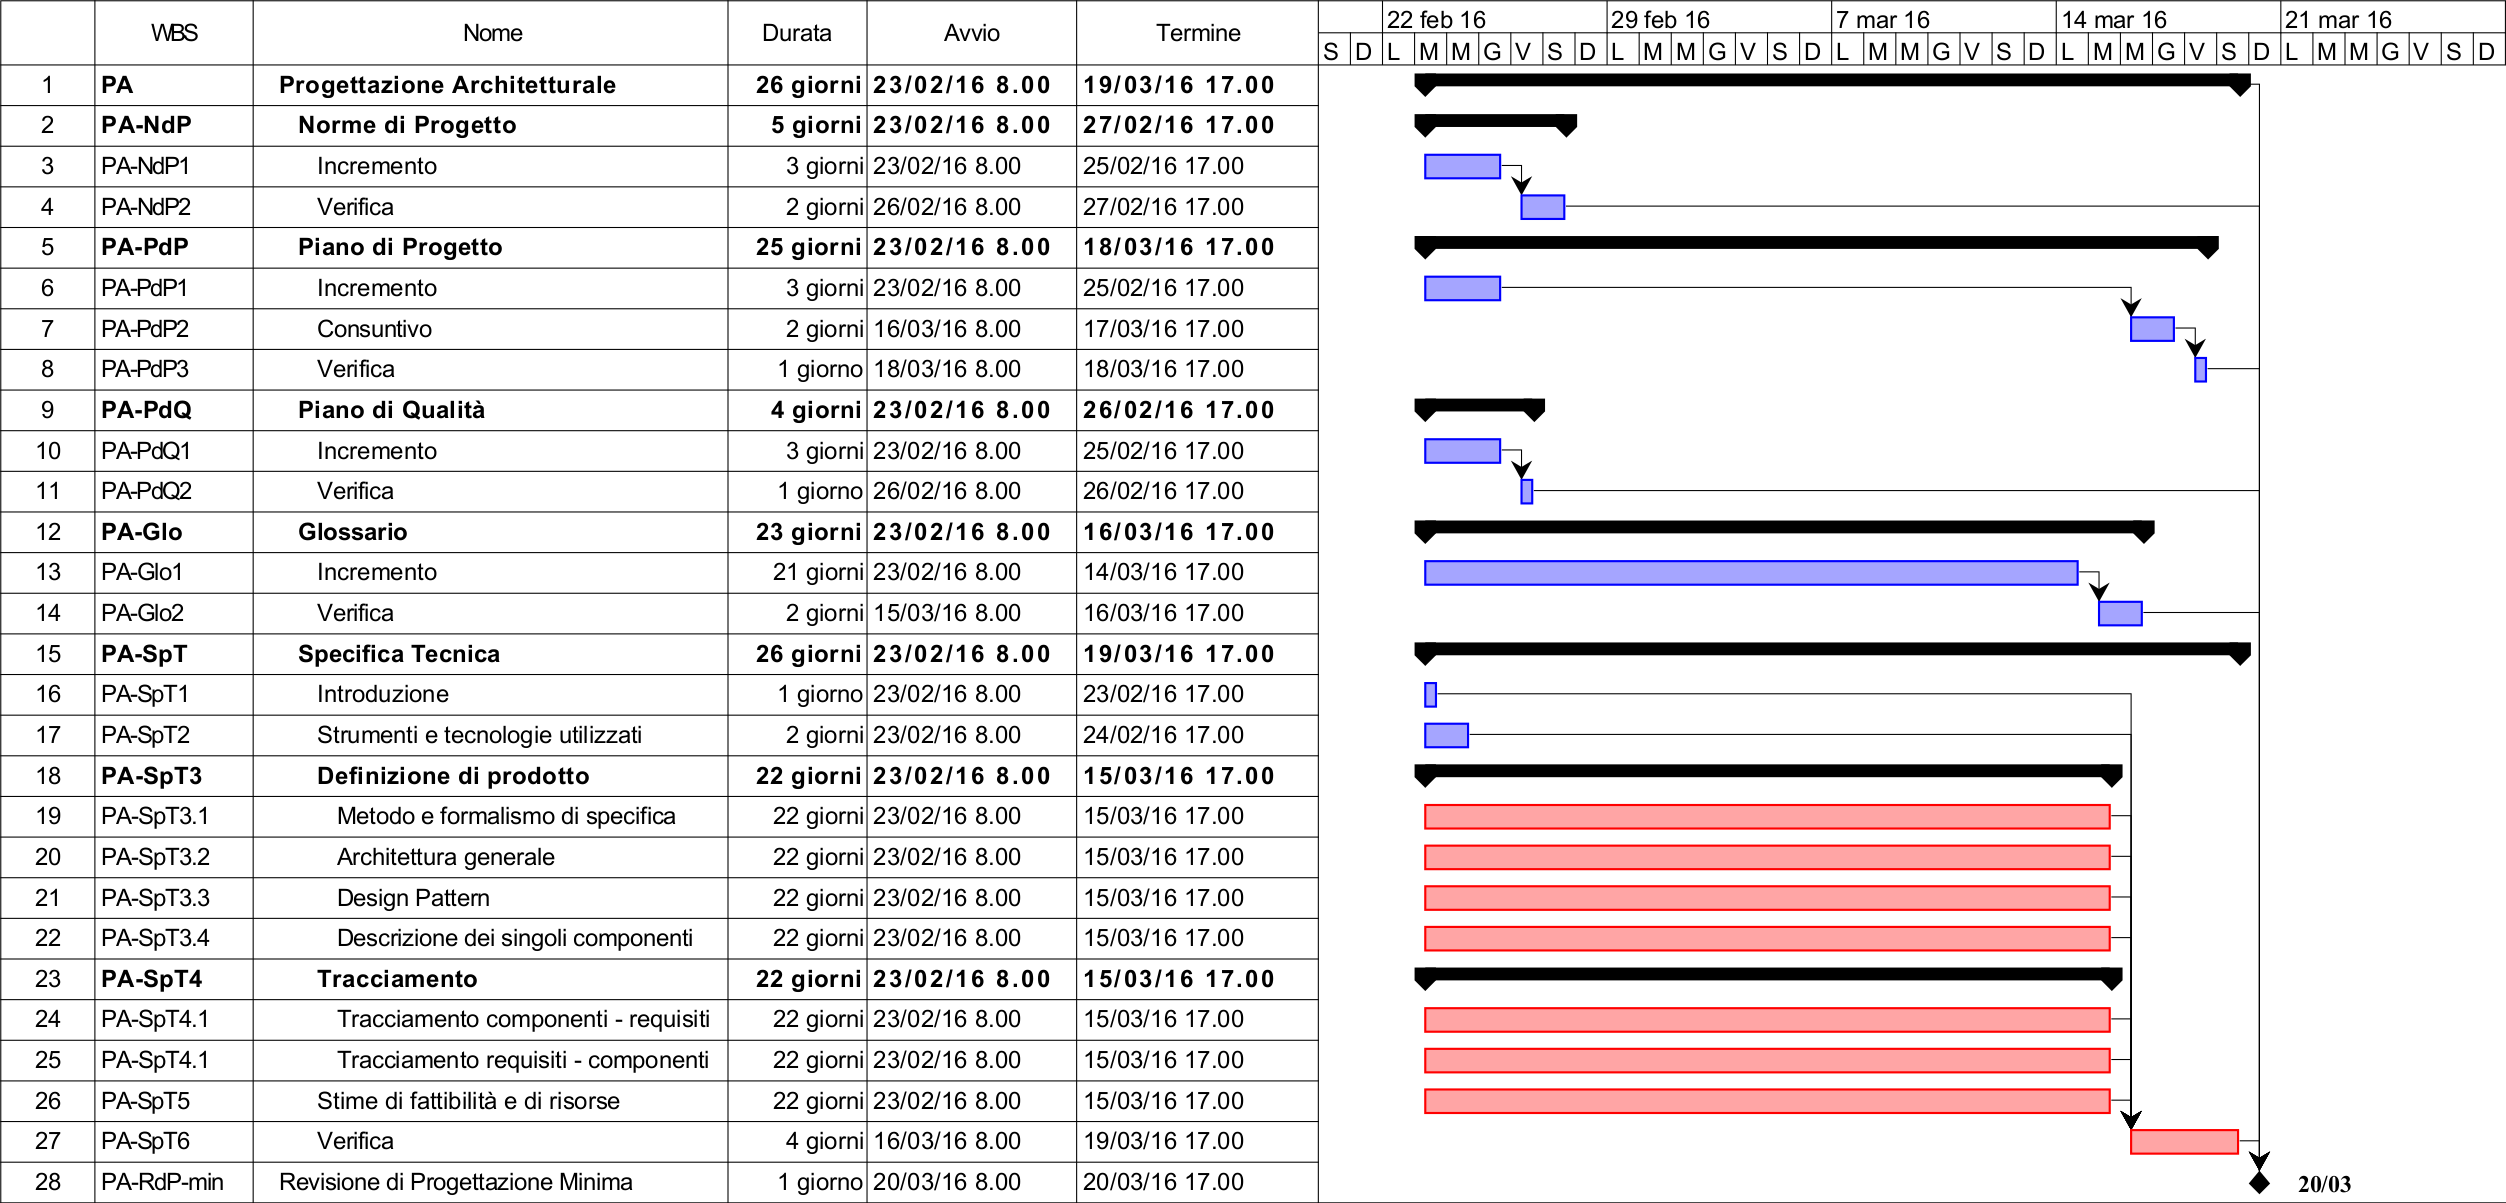
\includegraphics[keepaspectratio = true, width=15cm]{immagini/PdP_ProgettazioneArchitetturaleGantt.png}
\end{center}
\begin{figure}[h]
	\caption{Diagramma di Gantt relativo al periodo di Progettazione Architetturale.}\label{etichetta}
\end{figure}

\subsubsection{Progettazione di Dettaglio}
\textbf{Periodo:} dal 21 Marzo all'11 Aprile 2016. \\
Questo periodo, di Progettazione di Dettaglio, inizia dopo il periodo di Progettazione Architetturale e si conclude con la consegna dei documenti per la Revisione di Progettazione. L'obbiettivo di questo periodo è la stesura, in modo dettagliato, dell'intero sistema, specificando in modo approfondito il comportamento e l'iterazionetra tra i vari componenti. \\
Prevede di svolgere le seguenti attività:
\begin{itemize}
	\item Redigire il documento di \textbf{\DDP}: il \Prog deve descrivere il comportamento e le iterazioni tra i vari componenti del sistema basandosi sul documento di \ST.  
	\item Incrementare i documenti di \textbf{\NdP},\textbf{\PdP}, \textbf{\PdQ}, \textbf{\ST} e \textbf{Glossario}.
	\item Verifica di tutti i documenti sopraccitati.
\end{itemize}
\begin{center}
	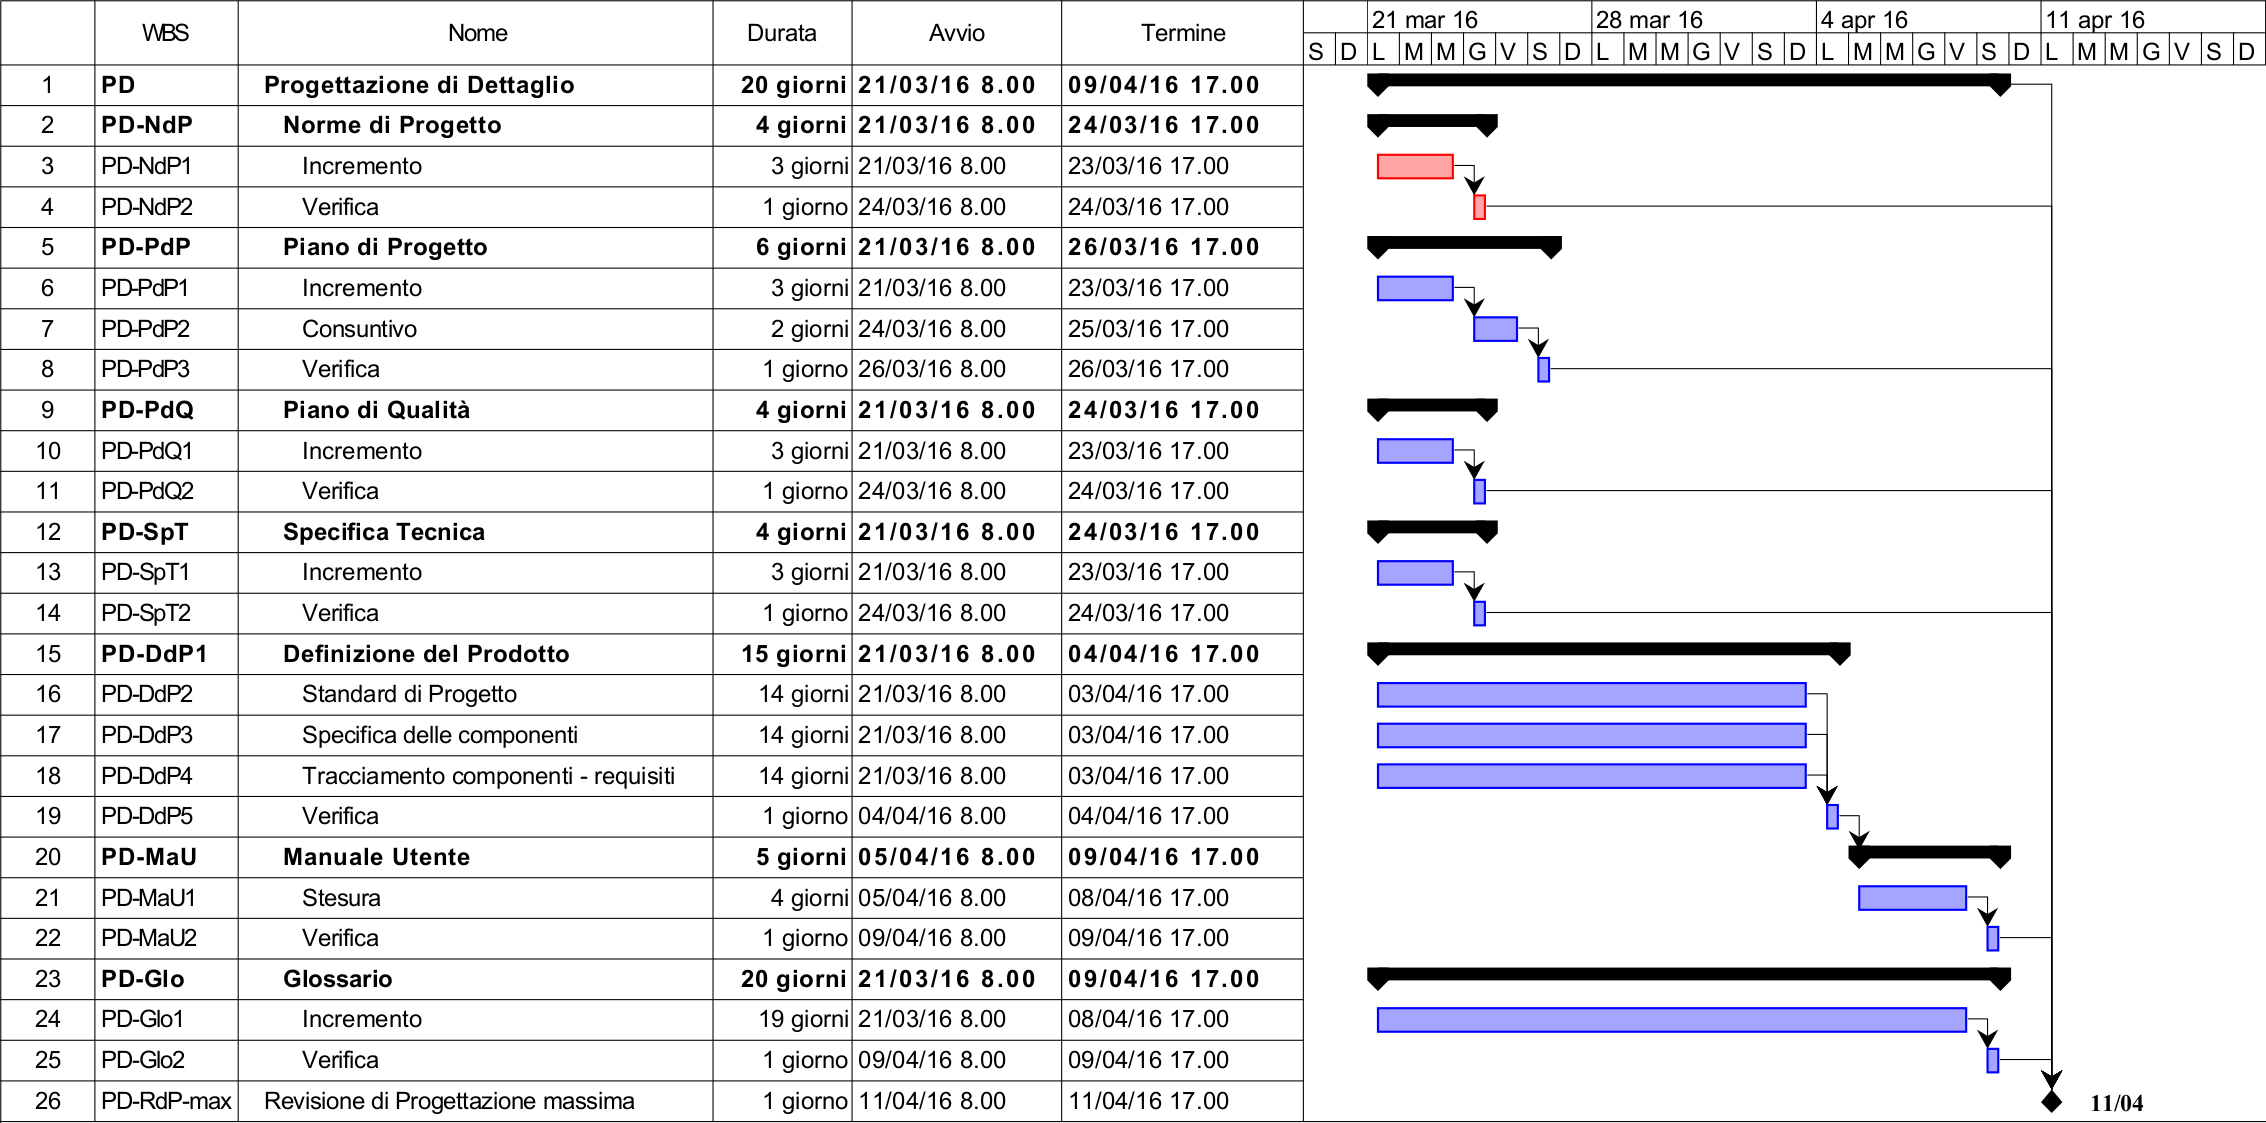
\includegraphics[keepaspectratio = true, width=15cm]{immagini/PdP_ProgettazioneDiDettaglioGantt.png}
\end{center}
\begin{figure}[h]
	\caption{Diagramma di Gantt relativo al periodo di Progettazione di Dettaglio.}\label{etichetta}
\end{figure}

\subsubsection{Codifica}
\textbf{Periodo:} dal 19 Aprile 2015 al 16 Maggio 2015. \\
Questo periodo, di Codifica, inizia dopo il periodo di Progettazione di Dettaglio e si conclude con la consegna del prodotto alla Revisione di Qualità. L'obbiettivo in questo periodo è di consegnare un prodotto qualificato e prevede di svolgere le seguenti attività:
\begin{itemize}
	\item   
	\item Incrementare i documenti di \textbf{\NdP},\textbf{\PdP}, \textbf{\PdQ} e \textbf{Glossario}.
	\item Verifica di tutti i documenti sopraccitati.
\end{itemize}
\begin{center}
	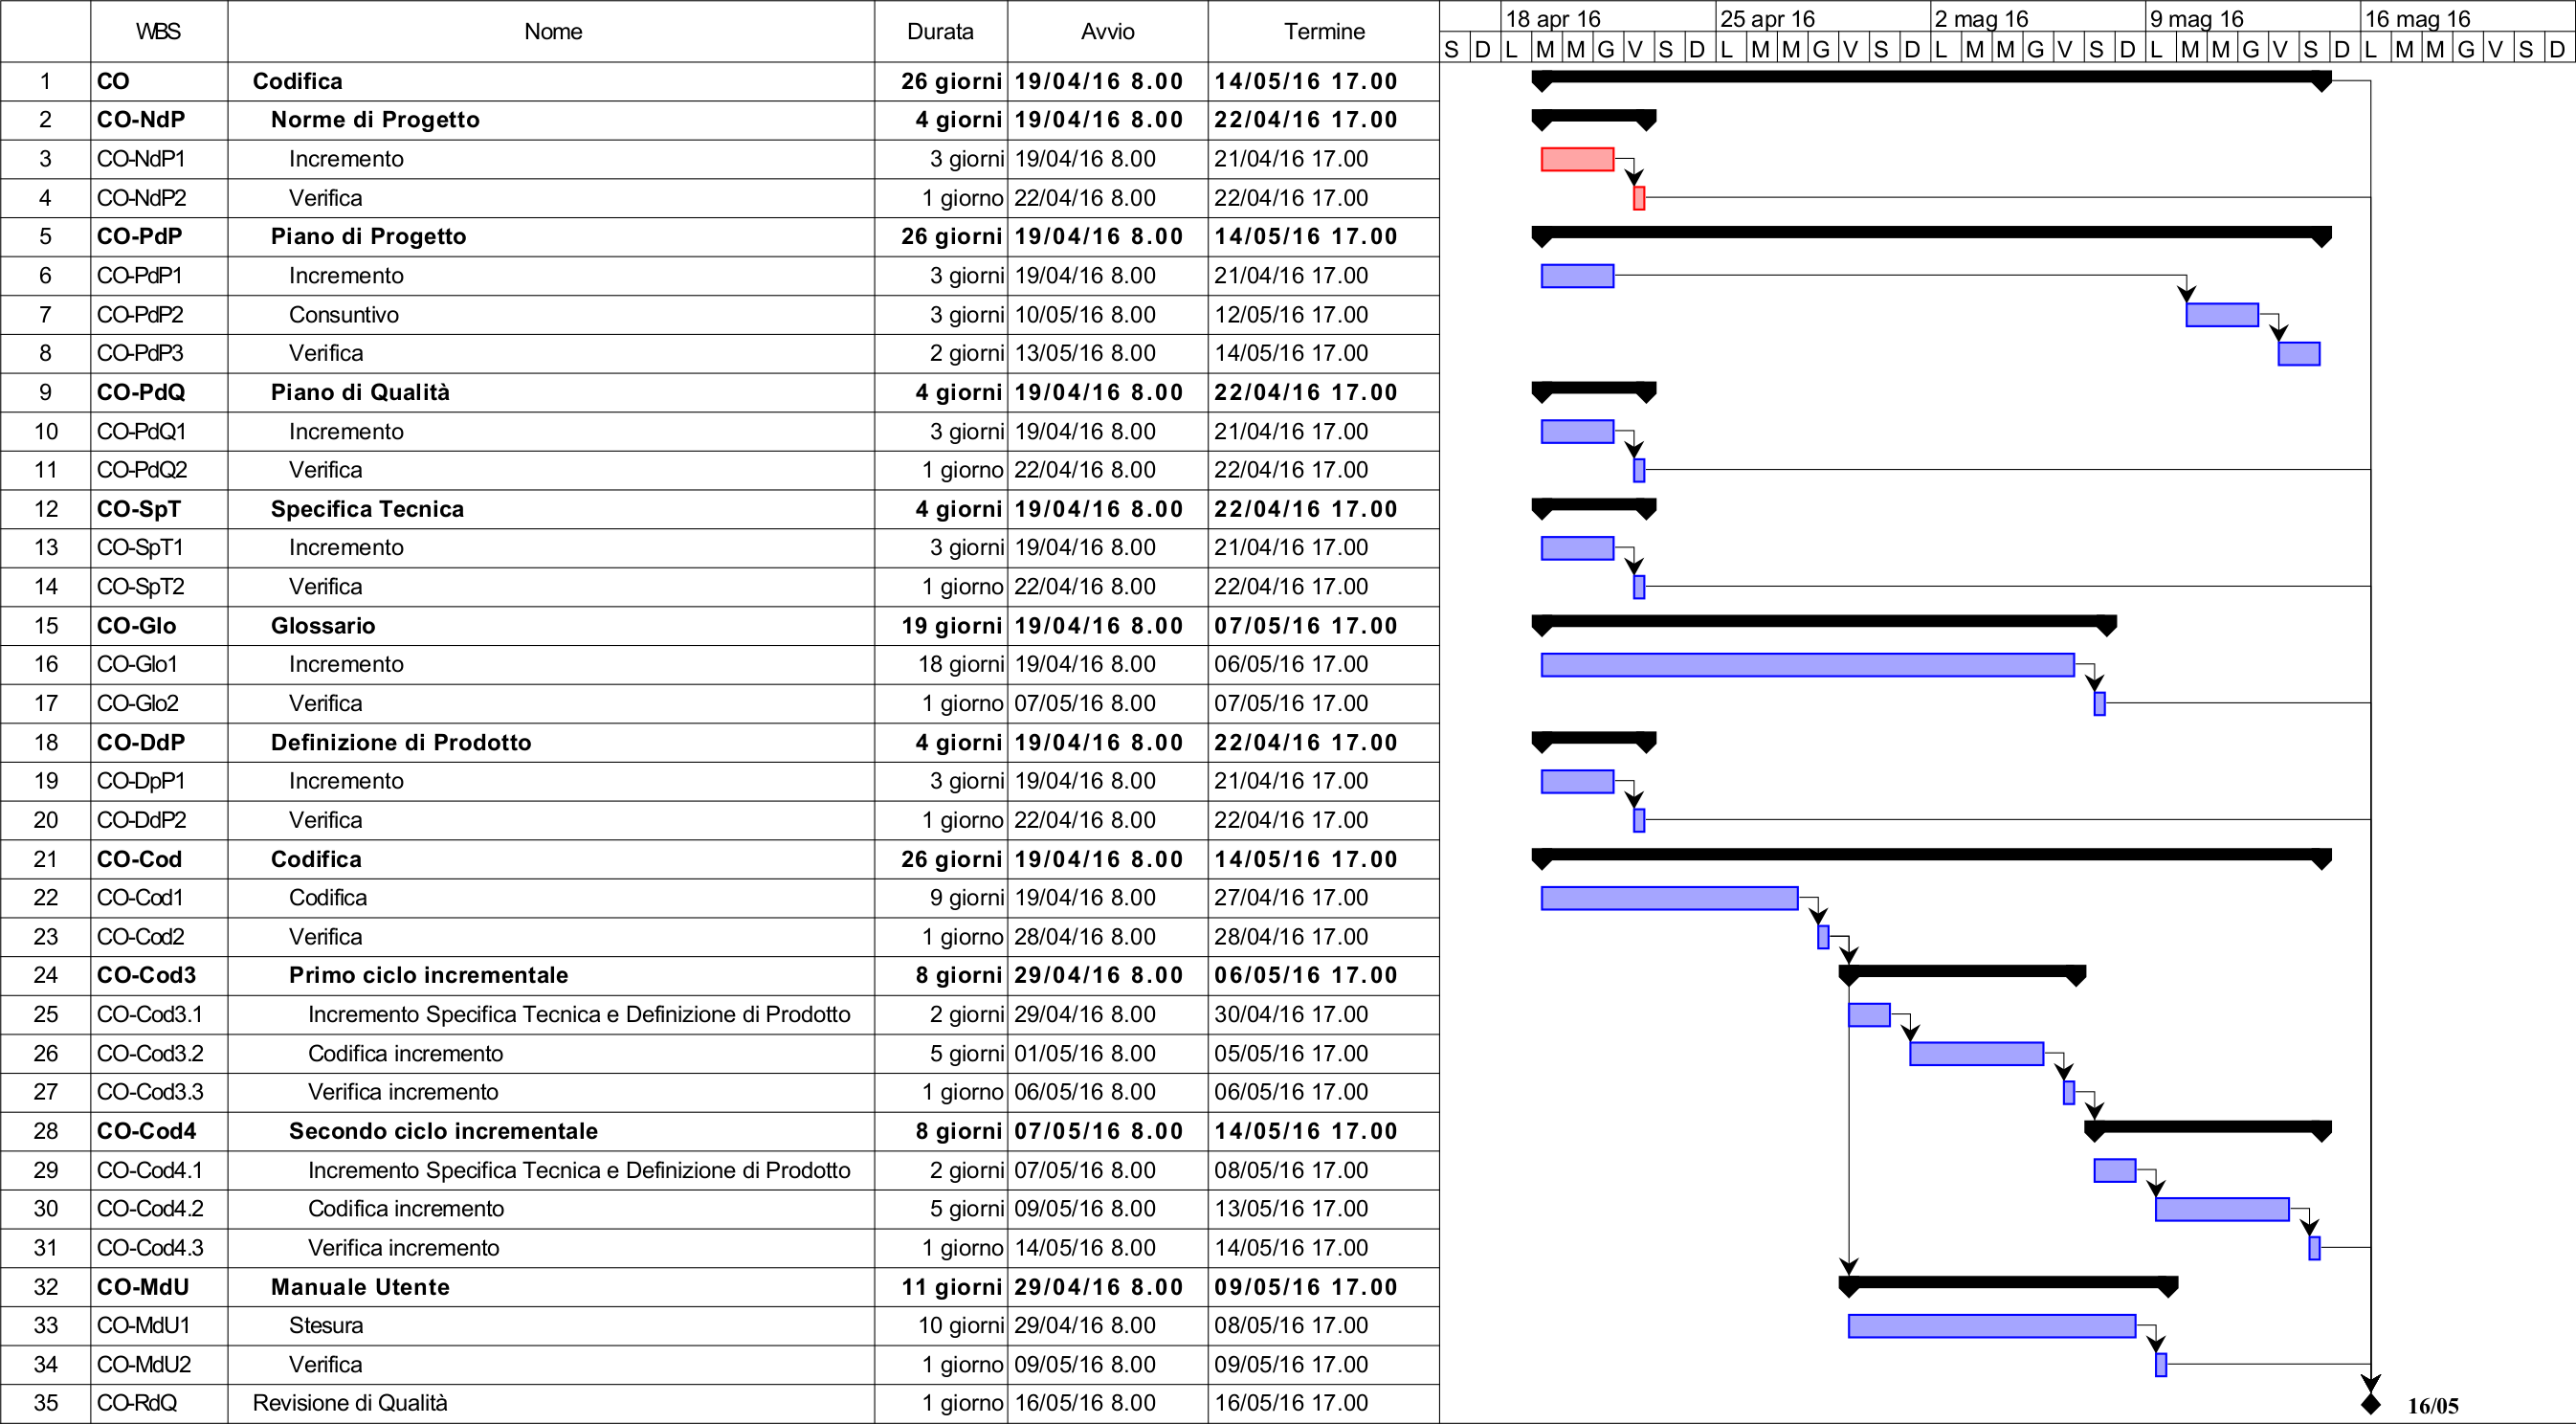
\includegraphics[keepaspectratio = true, width=15cm]{immagini/PdP_CodificaGantt.png}
\end{center}
\begin{figure}[h]
	\caption{Diagramma di Gantt relativo al periodo di Codifica.}\label{etichetta}
\end{figure}

\subsubsection{Verifica e Validazione}
\textbf{Periodo:} dal 24 Maggio 2016 al 10 Giugno 2016. \\
Questo periodo, di Verifica e Validazione, inizia dopo il periodo di Codifica e si conclude con la consegna del prodotto alla Revisione di Accettazione. In questo periodo vengono effettuati tutti i test necessari per garantire che il prodotto soddisfi tutti i requisiti dell'\AdR.  
Le attività sono di:
\begin{itemize}
	\item   
	\item Incrementare i documenti di \textbf{\MU},\textbf{\NdP},\textbf{\PdP}, \textbf{\PdQ} e \textbf{Glossario}.
	\item Verifica di tutti i documenti sopraccitati.
\end{itemize}
\begin{center}
	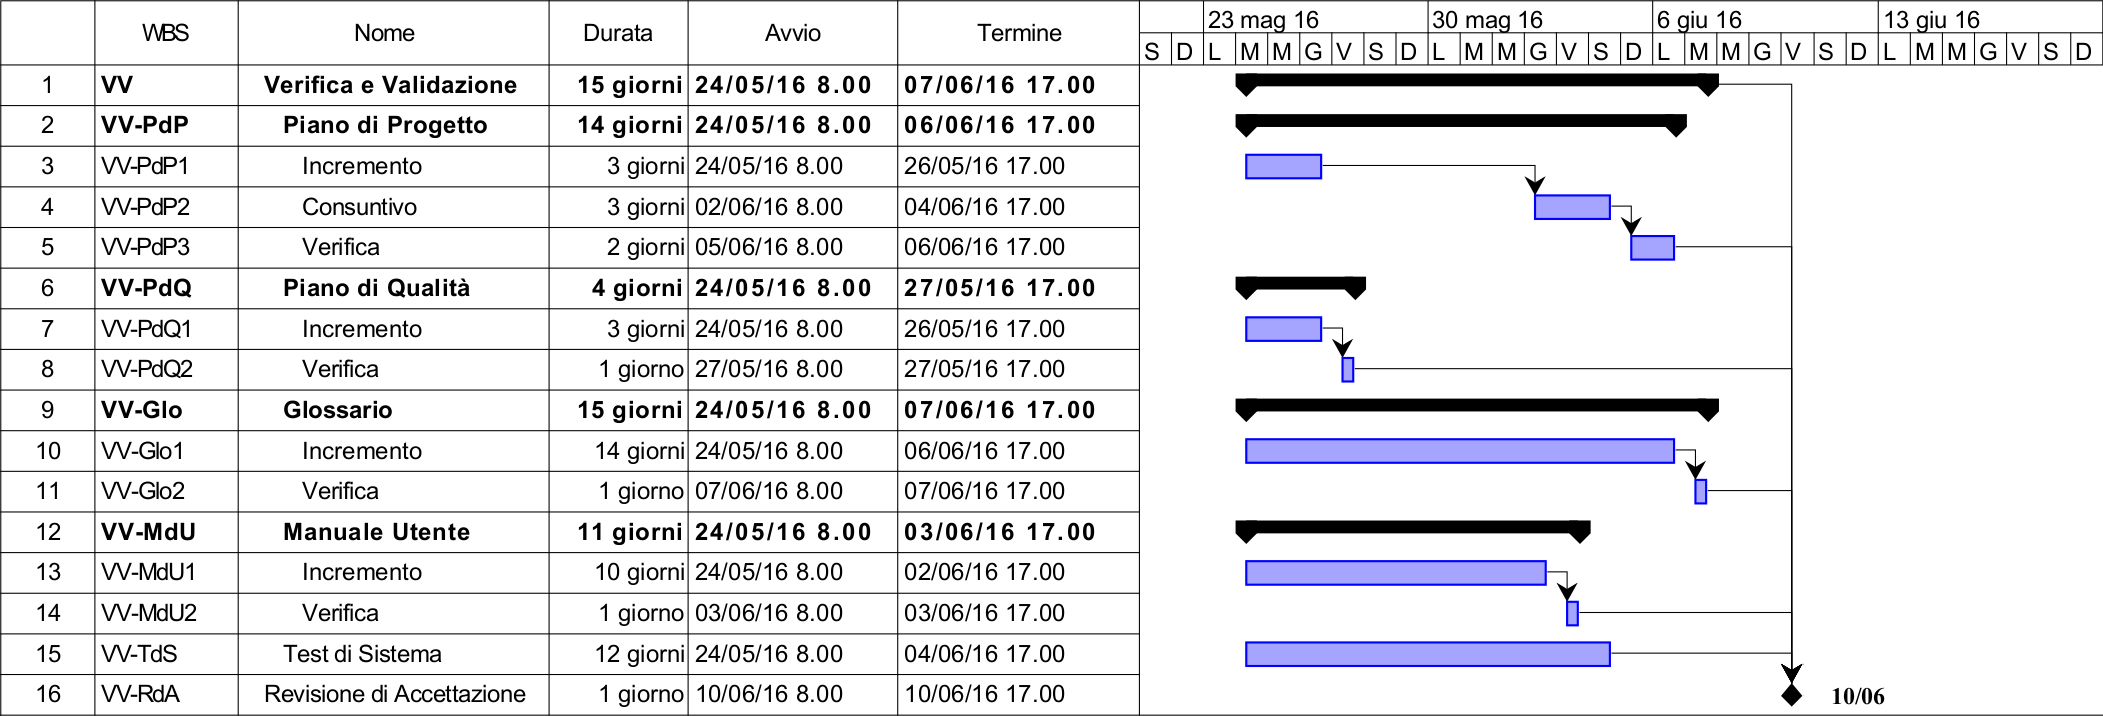
\includegraphics[keepaspectratio = true, width=15cm]{immagini/PdP_VerificaEValidazioneGantt.png}
\end{center}
\begin{figure}[h]
	\caption{Diagramma di Gantt relativo al periodo di Verifica e Validazione.}\label{etichetta}
\end{figure}